% Datei: Documents/rennvelo/trainingslager/main.tex
% Begonnen: 14.11.2015 
%
% Einteilung des Paperformates, des Satzspiegels und eine Bindekorrektur
\documentclass[a4paper,DIV13,BCOR0cm,draft=TRUE]{scrartcl}

% Sprach-Einstellungen
% babel ermöglicht die Verwendung verschiedener Sprachen, z.B. in Zitaten.
% Können mit \selectlanguage{english} resp. \selectlanguage{ngerman}
% umgestellt werden. Dabei ist die zuletzt eingestellte Sprache die
% Grundsprache und die Sprache der Bezeichner ("Inhaltsverzeichnis",
% "Abbildung") fest. Die Bezeichner können im Dokumentteil noch geändert
% werden (z.B. \renewcommand*\contentsname{Inhalt}). inputenc erlaubt die
% direkte Eingabe von Sonderzeichen, insbesondere deutscher Umlaute. Durch
% \usepackage[T1]{fontenc} werden von LaTeX Fonts in westeuropäischer
% Codierung verlangt. Dies führt zu einer verbesserten Trennung für
% westliche Sprachen. Zudem wird die Standardschrift von Computer Modern zu
% European Computer Modern umgeschaltet.
\usepackage[english,ngerman]{babel}
\usepackage[utf8]{inputenc}
\usepackage[T1]{fontenc}

% Problem, ein Hyphen in einem Wort (z.B. "Borderline-Persönlichkeitsstörung") verhindert,
% dass das Wort weiter getrennt wird.
\hyphenation{Trai-nings-la-ger}
\hyphenation{Renn-rad}
\hyphenation{Renn-ve-lo}

% Schrift
\usepackage{lmodern}    % Schrift "Latin Modern" laden
% Folgende Schrift-Optionen für serifenlose resp. Schreibmaschinenschrift aktivieren.
% \renewcommand*\familydefault{\sfdefault} % Serifenlose Schrift
% \renewcommand*\familydefault{\ttdefault} % Schreibmaschinenschrift

% Typographische Feinheiten
\usepackage{typearea}   % Einstellung des Satzspiegels, siehe Latex Hacks, Hack #31
\usepackage{mdwlist}    % Für enger gesetzte Listen
\usepackage{booktabs}   % schönere Tabellen, siehe WAsmL, p. 124

% Bietet mehr Kontrolle über Kopf- und Fusszeile
% Infos und Tutorial: https://www.ctan.org/pkg/fancyhdr
\usepackage{fancyhdr}
\pagestyle{fancy}

\usepackage{units}
\usepackage{gensymb}

% Die Option dvipdfmx und das Paket bmpsize verhindern
% die Fehlermeldung von latex:
% "cannot determine size of graphic"
% XXX: die Option dvipdfmx in graphicx hat bewirkt, dass Bilder nicht mehr angezeigt wurden.
\usepackage[]{graphicx}
\usepackage{bmpsize}

\usepackage{babelbib}
\usepackage{url}		% wird von babelbib gebraucht
\usepackage{apacite}
%\usepackage{hyperref}

\setcounter{secnumdepth}{1}

% Als Schweizer musste diese Option einfach sein.
\newcommand{\rv}{Rennvelo}
%\newcommand{\rv}{Rennrad}

\newcommand{\tlzh}{TLzH}
\newcommand{\Tlzh}{Trainingslager zu Hause}

\begin{document}

% Neudefinition einiger Bezeichner
\renewcommand*\contentsname{Inhalt} % Standart: Inhaltsverzeichnis
\renewcommand*\refname{Quellen} % Standart: Literaturverzeichnis

% \titlehead{}
\lhead{\tlzh}

% \subject{<+Thema+>}
\title{\rv-\Tlzh{} (\tlzh)}
\author{Marco Strehler}

%\publishers{}
\date{02.\,Februar\,2016}

\maketitle
%\clearpage

\begin{abstract}
Diese Zusammenstellung enthält Tipps zur Vorbereitung und Durchführung eines einwöchigen \rv"=Trainingslager zu Hause (\tlzh).
Dabei werden die Vor- und Nachteile erörtert im Vergleich zu einem konventionellen Trainingslager
(typischerweise fremdorganisiert und in mediterranen Regionen). 
Dies mit dem Ziel eines optimalen Resultates im Verhältnis zur aufgewendeten Zeit und anfallenden Kosten.
\end{abstract}

\tableofcontents
\section{Einleitung}

Ein Trainingslager (TL) im Frühling dient dazu
schon früh stabile Grundlagen für die anstehende \rv"-Saison zu legen.
Neben dem körperlichen Training kann man sich in einem TL auch mit anderen Themen rund um das Training beschäftigen.
Beispiele sind: Ernährung, Regeneration, \rv"=Technik oder Radrennhistorie.
Durch eine solche Immersion in die Materie wird die Motivation weit über das TL hinaus gestärkt.

Wird von einem Trainings\textsl{lager} gesprochen, impliziert das ein Ortswechsel.
Typischerweise an einen Ort, wo Frühling ist, wenn in Nord- und Mitteleuropa noch Eis und Schnee herrscht.

In der Regel wird dazu ein Pauschalangebot mit Hotel, geführten Trainingstouren und Möglichkeit der \rv-Miete.
Etwas luxuriösere Angeboten bieten noch Trainingsplanung, Begleitfahrzeug, Schrauberplatz und Massage.

Es gibt m.E. jedoch wenig wirklich objektive Gründe, als Nicht"=Profi für ein TL zu verreisen.
Umso mehr, als ein solches TL sich prima zu Hause durchführen lässt.
Ich bin überzeugt, dass ein \tlzh{} mehr Vor"= als Nachteile hat und genau so viel Spass macht.
Die folgende Zusammenstellung von Tipps und Hinweisen soll helfen, die Vorteile gut zu nutzen und allfällige Nachteile
auszugleichen.

% Hier kommt dann noch eine Inhaltsangabe der Kapitel.
% Im Abschnitt \ref{sec:wiesozuhause} beschreibe ich die Vor- und Nachteile eines \tlzh{}.

\section{Wieso ein Trainingslager zu Hause?}
\label{sec:wiesozuhause}

\subsection{Vorteile eines \tlzh}

Der augenscheinlichste Vorteil:
ein \tlzh{} kommt \emph{wesentlich günstiger} als ein TL an einer der üblichen Destinationen.
Die Preise für fremdorganisierte TL unterscheiden sich stark
und sind abhängig von der Hotel"=Qualität und dem gebotenen Service.
(für den von vielen angebotene Klassiker Mallorca siehe Tabelle \ref{tab:preisvergleich}.
Zu den Kosten des TL kommt der der Flug, allenfalls Transport des \rv{} oder dessen Miete vor Ort.
Die Mitnahme des eigenen Fahrrades kostet bei der Swiss in Europaflügen CHF 60 (EUR 50) und bei Interkoninentalflügen CHF 120 (EUR 100)
\cite{swiss2016fahrradmitnahme}. Die Preise anderer Anbieter sind vergleichbar.
Bei Mitnahme des eigenen Rades mit dem Flieger muss allenfalls ein Transportbehälter gekauft oder gemietet werden.
Die Preisspanne in einem Vergleich von 4 Radkoffern und 6 Radtaschen in der Zeitschrift RoadBIKE ging von EUR 300 bis 800
\cite{Brunker2015radkoffer}.
Das ist ein Haufen Schotter.

\begin{table}
  \centering
  \begin{tabular}{lrl}
    \toprule
        Anbieter"=Website & CHF/Euro & Bemerkungen \\
    \midrule
        \url{hoechstform.ch} & 1500/\textsl{1357} & Frühbuch"=Preis, 4"=Stern"=Hotel, Wellness"=Anlage \\
        \url{www.champions-training.de} & \textsl{618}/559 & im DZ, 4"=Stern"=Hotel, Wellness"=Anlage \\
        \url{www.huerzeler.com} & 645/\textsl{584} & incl. Flug ab Zürich od. Basel\\
        \url{www.radsport-mallorca.de} & 495/445 & im DZ \\
        \url{www.kollerbike.ch} & 413/\textsl{373} & 3"=Personen"=Appartement, 3"=Stern"=Hotel \\
    \bottomrule
  \end{tabular}
  \caption{Preisübersicht Februar 2016 für eine Woche Rennrad"=Training in Mallorca,
    von deutschen und schweizerischen Anbietern.
    Jeweils unter Berücksichtigung des günstigsten Angebotes.
    Wenn nichts angegeben sind die Preise ohne Flug und ohne Miet"=Rennrad.
  Preise in kursiv sind jeweils von der anderen Währung umgerechnet.}
  \label{tab:preisvergleich}
\end{table}

% Hier noch: Verhältnis gefahrener Trainingskilometer zu aufgewendetem Geld, bzw. aufgewendeten Ferientagen.

Doch für die meisten noch knapper als Geld ist heute Zeit.
Bei einem TL in einem anderen Gegend von Europa muss realistischerweise für Hin- und Rückreise je einen Tag gerechnet werden.
Zwei wertvolle Tage, die man in irgenwelchem Flugzeug oder Transferbus und nicht im Sattel sitzt?
Da blutet das Herz.

Auch ein gut ausgestattetes Hotel bietet nicht die gleich gute Infrastruktur, wie sie zu Hause zur verfügung steht.
Auch wer seinen Koffer mit Werkzeug füllt, wird das notwenige Teil im TL nicht dabei haben.
Dazu kommen noch allfällige Fachliteratur, Einkaufsmöglichkeiten (Fachgeschäfte) bei Bedarf und schneller Internetzugang.

Auch ein Trainingslager, dass unterschiedliche Leistungsstufen anbietet wird ein Kompromiss sein.
Vielleicht arbeitet man selber noch am Grundlagentraining, landet aber in einer Gruppe, die dauerend im Angriffsmodus fährt?
Nur zu Hause und alleine kann man die eigenen Trainingsziele perfekt umsetzen und muss keine Kompromisse bezüglich Art und Umfang des Trainings eingehen.

Der Zeitpunkt ist nicht von der Planung (oder freien Plätzen)des Anbieters abhängig, sondern kann optimal gewählt werden.
Der Abschnitt \ref{sec:richtigezeit} widmet sich der Frage nach dem richtigen Zeitpunkt.

Allenfalls neu entdeckte Touren am Wohnort können auch über das Traininglager hinaus in das Repertoire integriert werden.
Dadurch kann die Nachhaltigkeit sowie auch die Motivation über das ganze Jahr hinaus gesteigert werden.

\subsection{Nachteile eines \tlzh}

Dass mit dem Training für die Saison aufgrund der klimatischen Verhältnisse am Trainingsort früher begonnen werden kann,
kann umgekehrt natürlich als Nachteil für ein \tlzh{} betrachtet werden.

Ein \tlzh ist darüber hinaus -- weil weniger exotisch -- allenfalls weniger motivierender als ein Trainingscamp auf Mallorca, Malta oder in der Toscana.

In einem Trainingslager hunderte von Kilometern zu Hause fällt die Abgrenzung zum Alltag weniger schwer und
man kann sich ganz auf die gliebte Sache konzentrieren.
Die alltäglichen Pflichten -- Einkaufen, Kochen, Bett machen -- werden einem in einem Hotel abgenommen.

Es fehlen zu Hause das gewisse \emph{Profi"=Equipment}: kein Guide, kein Begleitwagen, keine Massage im Hotel.

Das Fahren in der Gruppe kann nicht speziell geübt werden.

Bei der Hausrunde fehlt der soziale Kick, der mit einer Woche Radfahren in einer südlichen Feriendestination verbunden ist.
Insbesonderen die <<weichen Fakten>>, welche ein Traininglager im Süden ausmachen werden bei \citeNP{Friedrich2008trainingslager}
schön beschrieben.

Beobachtet man die Diskussionen auf \url{http://www.rennrad-news.de/forum} dann bekommt man nicht den Eindruck,
dass es bei der Wahl des geeigenten Hotels für ein Trainingslager hauptsächlich um harte Trainingsaspekte geht.
Es werden Dinge genannt, die auch für einen Strandurlaub gelten könnten:
<<sauber>>, <<Essen ausgewogen und gut>>, <<Abends doch ein bißchen Bespassung>> \cite{tka19762010hotel},
<<ruhig>>, <<Wellness"=Bereich>>, <<Personal ist freundlich, zum Teil deutschsprachig>> \cite{garfield22011hotel},
<<Halbpension und Bettenaufschüttelservice>> und <<Flüssigkeitsausgleich>> \cite{orteb2011hotel}.
Das ist nicht falsch und soll so sein. Es bestärkt aber die Vermutung, dass es bei einem TL im Süden mehr 
um den Ferienaspekt als um frühe Performance geht.

\section{Wann ist die richtige Zeit?}
\label{sec:richtigezeit}

Der Hauptgrund eines TL im Süden ist das Klima.
Daran gibt es nichts zu rütteln: Temperaturen über \unit[10]{\degree C} gibt es in der Schweiz, Deutschland oder Oesterreich
drei Monate später als in den bevorzugten südlichen TL"=Destinationen (Tabelle \ref{tab:tempmax}).
Interessant dabei ist aber, dass der Februar in unseren Breitengraden
wohl kalt aber sehr trocken ist.
Der Februar hat im Mittel \textit{am wenigsten Niederschläge} von allen Monaten (Tabelle \ref{tab:niederschlag}).
Der März ewas milder und immer noch sehr trocken.
Mit geeigneter Bekleidung ist also ein \rv"=Training im Februar oder März
in unseren Breitengraden durchführbar.
Natürlich kann es bei uns über das ganze Jahr eine Woche durchregnen, aber spätestens im Mai gilt ein
lokales Training auch für Frostbeulen als problemlos möglich \cite{capricorn2015ausland,raimi272015wetter}.

\begin{table}
        \centering
        \begin{tabular}{lcccccc}
                \toprule
                 Land & Jan & Feb & März & Apr & Mai & Jun \\
                 \midrule
                 Oesterreich     & \textit{-1,3} & \textit{1,2} & \textit{5,7} & 10,5 & 15,1 & 18,3 \\
                 Deutschland    & \textit{2,1} & \textit{3,5} & \textit{7,4} & 11.7 & 16,8 & 20,0 \\
                 Schweiz        & \textit{3,8} & \textit{5,3} & \textit{9,4} & 13,5 & 17,6 & 21,4 \\
                 Italien        & 11,2 & 12,3 & 14,6 & 17,9 & 22,2 & 26,0 \\
                Mallorca        & 14,0 & 15,0 & 17,0 & 19,0 & 22,0 & 26,0 \\
                Sardinien   & 14,1 & 14,7 & 16,1 & 18,4 & 22,3 & 26,3 \\
                Sizilien    & 14,5 & 14,8 & 16,0 & 18,3 & 22,4 & 26,4 \\
                Malta       & 15,2 & 15,5 & 16,7 & 19,1 & 23,3 & 27,5 \\
                 Zypern         & 15,7 & 16,3 & 20,1 & 24,3 & 29,6 & 23,3\\
                 Spanien        & 15,8 & 16,8 & 18,7 & 20,0 & 22,6 & 25,8 \\
                 \bottomrule
        \end{tabular}
        \caption{
            Mittleres Temperaturmaximum Januar bis Juni \protect\cite{rtl2015klima}.
            Die Zeilen sind ansteigend nach der Temperatur im Januar sortiert.
            Temperaturen unter \protect\unit[10]{\degree C} sind kursiv gesetzt.
            }
        \label{tab:tempmax}
\end{table}


\begin{table}
        \centering
        \begin{tabular}{lcccccc}
                \toprule
                 Land & Jan & Feb & März & Apr & Mai & Jun \\
                 \midrule
                 Oesterreich     & 85,2 & \textit{78} & 88,8 & 101 & 115,6 & 141,2 \\
                 Deutschland    & 54,1 & \textit{44,6} & 52,1 & 57,4 & 69,2 & 81,3 \\
                 Schweiz        & 73,7 & \textit{72,7} & 84,7 & 102,3 & 126 & 128 \\
                 \bottomrule
        \end{tabular}
        \caption{
                Mittlere Monatssumme des Niederschlages [mm] Januar bis Juni \protect\cite{rtl2015klima}.
                Der durchschnittliche trockenste Monat (kursiv) ist der Februar.
            }
        \label{tab:niederschlag}
\end{table}

Für den Zeitpunkt ein möglichst optimales Trainingscamp sollten:
schon ein Grundlagentraining vorhanden sein (ca. 1000 km, entsprechen 4 - 8 Wochen)
Nach dem Trainingscamp die Möglichkeit vorhanden sein, das erreichte Niveau aufrecht zu erhalten und zu nutzen.

Strassenzustand:
zu Beginn des Frühlings sind die Strassen durch Split, Salz und allenfalls liegengebliebener Schnee nicht ideal.
Um Salzschäden zu vermeiden soll das Rad nach der Ausfahrt auch mit Wasser abgespühlt werden.

Vorteilhaft für das Ferientage"=Budget ist eine Woche,
die bereits offizielle Feiertage enthält.
So können mit wenig eingesetzten Urlaubstage eine schöne Anzahl
aneinanderhängender Trainingstage gewonnen werden.
Der Klassiker ist hier die Karwoche,
in der man mit vier eingesetzten Ferientagen gleich 10 Tage am Stück zum Trainieren hat
(Tabelle \ref{tab:karwoche}).
Der Nachteil an der Karwoche ist, dass diese in der Regel im April liegt,
der deutlich mehr Niederschläge hat.
\footnote{Ein kleiner Hinweis für Linux"=Anwender:
mit dem Terminalbefehl \texttt{ncal -e JJJJ} erhält man direkt das
Datum des Ostersonntages des entsprechenden Jahres. Also mit \texttt{ncal -e 2026}
den 5.\,April 2026.}

\begin{table}
        \centering
        \begin{tabular}{ccc}
                \toprule
                    Jahr & Wochen"=Nr. & Ferieneingabe (Sa -- Mo)\\
                \midrule
                    2016 & 12 & 19.03.16 -- 28.03.16 \\
                    2017 & 15 & 08.04.17 -- 17.04.17 \\
                    2018 & 13 & 24.03.18 -- 02.04.18 \\
                    2019 & 16 & 13.04.19 -- 22.04.19 \\
                    2020 & 15 & 04.04.20 -- 13.04.20 \\
                    2021 & 13 & 27.03.21 -- 05.04.21 \\
                    2022 & 15 & 09.04.22 -- 18.04.22 \\
                    2023 & 14 & 01.04.23 -- 10.04.23 \\
                    2024 & 13 & 23.03.24 -- 01.04.24 \\
                    2025 & 16 & 12.04.25 -- 21.04.25 \\
                \bottomrule
        \end{tabular}
        \caption{Daten der Karwoche.
            Für die direkte Eingabe der Ferien über die Wochennummer oder
            der konkrete Zeitraum des \tlzh{} vom Samstag vor der Karwoche bis Ostermontag.}
        \label{tab:karwoche}
\end{table}


\section{Trainingsplanung}

Grundsätzliches Vorgehen bei der Planung (modifiziert nach \citeNP{Beck2015}):

\begin{itemize*}
        \item Gesamtstunden 2 -- 2,5-fach des üblichen Pensums.
        \item Trainingstage in Blöcke von 2 -- 3 Trainingstagen plus einem Regenerationstag aufteilen.
        \item Die tägliche Trainingszeit jeweils um 0.5 Stunden steigern.
                Eine Alternative ist, jeweils den zweiten Tag im Block etwas kürzer zu gestalten,
                um am 3. Tag in sehr guter Form zu sein (z.B. 3:30\,h -- 3:00\,h -- 4:00\,h)
        \item Die tägliche Trainingszeit wird in jedem Block um 0.5 Stunden gesteigert.
\end{itemize*}

\begin{table}
        \centering
\begin{tabular}{lll}
    \toprule
    & Dauer [h] & Trainingsbereich \\
    \midrule
        Tag 1 & 3:00 & GA1"=Bereich \\
        Tag 2 & 3:30 & GA1"=Bereich \\
        Tag 3 & -- & Regeneration \\
        Tag 4 & 3:30 & GA1/2"=Bereich \\
        Tag 5 & 3:00 & GA1/2"=Bereich \\
        Tag 6 & 4:00 & GA1/2"=Bereich \\
    \bottomrule
\end{tabular}
\caption{Beispiel für die Gestaltung eines Trainingslagers mit 6 Trainingstagen \protect\cite{Beck2015}.}
        \label{tab:beispielplan}
\end{table}

Eine Alternative wäre, das TL nicht im Rahmen des Grundlagentrainings zu sehen,
sondern als Ausbautraining, resp. ganz konkret in die Wettkampfvorbereitung einzubauen.
Das Trainingslager wird also nicht für die Grundlage sondern für das <<Peaking>> eingesetzt.
Damit (von englisch \textit{peak} für Gipfel) wird gezielte Optimierung der Form auf einen Wettkampf bezeichnet.
Voraussetzung dazu ist natürlich, dass das Grundlagentraining vorgängig auf der Rolle geleistet wurde.
\citeNP{Beck2011} stellt ein 6"=Wochen"=Programm im Vorfeld eines Wettkampfs vor.
Ideal wäre hier, das TL in den Wochen 6, 5 oder 3 dieser Vorbereitungsphase zu legen.

\begin{itemize*}
        \item Woche 6 Grundlagen legen:
                Grundlagenausdauer mit langen und lockeren Einheiten.
                Eine davon soll mindestens so lange dauern wie der geplante Wettkampf.
        \item Woche 5 Intensität erhöhen:
                Intensivere Intervalle im GA2"=Bereich:
                Dazu Trittfrequenz"=Training mit 100 Umdrehungen pro Minute.
                Die Anstrengenden Einlagen von 20--30 Minuten in Grundlagenausfahrten integrieren.
        \item Woche 4 Vorbereitung aufs harte Training:
                Grundlagenausdauer von kürzerer Dauer von 1.5 bis 2 Stunden
                um die Grundlage zu stabilisieren.
        \item Woche 3 Feinschliff:
                Intensives Training (HIT, Training am Berg, Sprint"=Intervalle) oder ein Vorbereitungswettkampf.
        \item Woche 2 Regeneration:
                Zwei bis drei lockere Runden. Regeneration mit Schlafen, Massage und Sauna.
        \item Woche 1 Rennen optimal vorbereiten:
                Spezielles Training: Dienstag 2h GA1, Mittwoch 2h GA1, Donnerstag 2h lockere Einheit, Freitag Ruhetag, 
                Samstag 1h GA1-Einheit mit 2mal 2 Minuten EB"=Training.

\end{itemize*}


\section{Streckenplanung}

Während einem \tlzh{} ist man frei. Entsprechend den Trainingszielen sollen die Strecken gewählt werden.

Ein Punkt, der bei der Planung der Strecke allenfalls ins Gewicht fällt,
sind die Unterschiede im Verkehr zwischen Wochentagen und Wochenende.
So sind Hauptstrassen, die man von Sonntagsausfahrten kennt plötzlich voller Laster.
Andererseits sind Ausflugziele besonders an den Wochenenden viel befahren.

Oft wird bei den TL ein Begleitfahrzeug angeboten.
Der Vorteil bei einem \tlzh{} ist allerdings, dass das Netz des öffentlichen Verkehrs bei uns
wesentlich dichter ist und das man bei einer nicht reparierbaren Panne oder totaler Erschöpfung
mitsamt dem \rv{} nutzen kann. Auch könnte man sich mit den eingesparten Kosten auch ein Taxi leisten.

 

\section{Tagesplanung}

Ein Vorschlag für eine Tagesplanung findet sich bei \citeNP{Boehme2016trainingstag}.

\begin{table}
  \centering
  \begin{tabular}{cll}
    \toprule
    Zeit & Tätigkeit & Bemerkungen \\
    \midrule
 08:00 Uhr & Frühstück & mindestens 2 Stunden vor dem Training frühstücken.\\
  09:30 Uhr & Radcheck & \\
  10:00 Uhr & Ausfahrt & bei 4 Stunden unterbrochen durch eine 15"=30"=minütige Pause \\
  15:00 Uhr & spätes Mittagessen & \\
  16:00 Uhr & Gymnastik & aufdehnen und strecken (z.B. mit Yoga) \\
  16:30 Uhr & Powernap & \\
  19:00 Uhr & Abendessen & \\
  22:00 Uhr & Schlafen & \\
    \bottomrule
  \end{tabular}
  \caption{Vorschlag für eine Tagesplanung. Wieso diese für ein \tlzh{} angepasst werden sollte im Text. }
  \label{tab:tagesplanboehme}
\end{table}


Wer allerdings sein TL in einer noch kühlen Jahreszeit durchführt, der Radelt mit obigem Programm
in Eiseskälte los und und ist zur wärmsten Tageszeit (Nachmittag) schon wieder zu Hause.
Obige Zeiteinteilung ist also perfekt für den Sommer, dass man zur heissesten Tageszeit seine Siesta machen kann.
Für Training bei uns in den Monaten Februar und März eigenen sich die Nachmittagsstunden besser.

\citeNP[Seite 873]{Weineck2010} empfielt, das Frühstück auf zwei
Teile aufzuteilen (z.B. 06:00 und 09:00 Uhr). Durch das 2. Frühstück
soll der Leistungsabfall am vormittag abgefangen und der Tiefpunkt am Mittag
abgemildert werden.

Weitere Feinheiten der Trainingsplanung wäre ein <<Splitting>> der Einheiten.
Das durchführen von mehreren Trainingseinheiten am Tag hat den Vorteile,
dass dem allenfalls schlechten oder kalten Wetter Rechnung getragen wird.
Auch können in zwei kürzeren Einheiten intensivere Einsätze geplant werden.
Auch gibt es einen doppelten Stimulus.
Dazwischen 2-4 Stunden Pause, am besten mit einer Schlafphase (Ausschüttung Wachstumshormon).

\section{Training in Kälte}

\subsubsection{Körperliche Adaption}
Ein \Tlzh{} im März oder April wirft die Frage nach Training in der Kälte auf.
Die Anpassung an die Kälte erfolgt beim Menschen vorwiegend durch Verhaltensänderung.
Trotzdem gibt es auch beim Menschen eine körperliche Adaption an Kälte \cite[S. 1032]{Weineck2010}.

\begin{itemize*}
        \item Nachlassen des Kälteempfindens
        \item Auftreten von Kältezittern bei tieferen Körperkerntemperaturen
        \item Steigerung des Grundumsatzes
        \item lokale Akklimationsion (Hände, Füsse) durch wiederholte Kälteexposition
\end{itemize*}

\subsubsection{Verhaltensanpassung}

Bezüglich Verhaltensänderung gibt es für Fahren bei Kälte im Netz und Fachzeitschriften massenweise Hinweise
\cite{Thomas2009rennradbuch, gcn2011winter,gcn2015winter, gcn2015wintermistakes,beck2015frostschutz}.

\begin{itemize*}
        \item Training:
                windgeschützte Route wählen (Wald),
                gegen den Wind losfahren und mit Rückenwind nach Hause <<treiben lassen>>,
                schweisstreibende Intervalle gegen Schluss des Trainings absolvieren,
                härter und kürzer trainieren,
                kurze Anstiege und kurze Abfahrten wählen,
                kurze Rundstrecken nahe zu Hause von 10 -- 20 km mehrfach absolvieren,
                bei Reparturstopp bei Gruppenausfahrten soll der Rest der Gruppe in Bewegung bleiben (Schlaufen fahren).
        \item Kleidung:
                Zwiebelschalenprinzip der Kleidung (mehrere Schichten sind effektiver),
                Zeitung oder Plastiktüte als Windschutz unter das Trikot schieben,
                Zehen mit einer <<Kappe>> aus Aluminium"=Folie vor Kälte schützen,
                Ueberschuhe oder ein altes Paar Socken (mit Loch für die Cleats),
                ein Paar dünner Gummihandschuhe über die \rv"=Handschuhe ziehen,
                Frischhaltefolie über den Helm gezogen,
                trockenes Ersatz"=Trikot für Kaffee"=Stopp.
        \item Ausrüstung:
                Isolierte Trinkflasche,
                Zwei Ersatzschläuche mitführen,
                Genügend Werkzeug mitführen.
                Verpflegung mitführen,
                Smartphone mit Gefrierbeutel vor Nässe (Schweiss) schützen.
        \item Rad:
                Reifendruck um 0.5 -- 1.0 bar reduzieren.
                Reifen regelmässig kontrollieren,
                All"=Wetter"=Reifen (z.B. Four Season von Continental, Durano von Schwalbe) montieren,
                kleine Akku"=Leuchten auch für den Tag,
                Reflektoren an Rad und Kleidung,
                Spritzschutz montieren,
                Reinigung und Schmieren des Bikes nach jeder Fahrt,

\end{itemize*}

\section{Regeneration}

Training muss Periodisiert werden. Ein umfangreiches Trainingspensum fordert eine entsprechende Regenerationsphase.
Es besteht die Gefahr, dass die Verpflichtungen des Alltags jedoch nicht ausreichend Raum für die entsprechend notwendige Regeneration lassen.
Hier gilt es, die Belastung in dieser Phase gering zu halten: Termine und Pendenzen sollen vor dem TL erledigt werden.

Es ist immer gut, wenn die Familie oder der Partner miteinbezogen wird.
So ein Camp ist ein kleiner Ego"=Trip. Der steht einem zu, soll aber auch in Familie und Partnerschaft eingebettet werden.
Vielleicht findet die Familie das ja auch toll und man verspricht sich, gegenseitig regelmässig bei solchen <<Camps zu Hause>> zu unterstützen.

Beim Schlaf sollte auf ein ausreichendes Pensum und Rhythmus geachtet werden.

Die Ernährung sollte dem Sport angepasst werden.

Das in der Umgebung angebotene Wellnessprogramm darf in dieser Trainingsphase ausreichend in Anspruch genommen werden.
Sei es Sauna \cite[S. 795]{Weineck2010}, Thermalbad.
Wer hart zu Hause trainiert, sollte sich auch den nötigen Luxus gönnen.
Alles, was hilft, schneller zu regenerieren und sich wieder fit für den nächsten Tag zu machen, sollte unternommen werden.

% \subsection{Open"=Window"=Phänomen}
% 
% Der Begriff des Open"=Window"=Phänomen beschreibt die immunologische Schwäche nach sportlicher Betätigung.
% 

\section{Nebenprojekte umsetzen}

Neben Trainieren, Essen, Schlafen bleibt noch etwas Zeit.
Diese kann genutzt werden, um Projekte rund um das \rv{} umzusetzen.

\begin{itemize}
        \item Einarbeitung ins Tracken von Routen.
        \item Sport"=Ernährung: Rezepte umsetzen, Riegel selber machen.
        \item Rennsport"=Geschichte: Bücher zum Thema Radrennsport lesen.
        \item Werkstatt: Aufbau einer eigenen Radwerkstatt (Schrauberecke).
                Dazu Literatur studieren und allenfalls eigenes kleines Projekt durchziehen.
        \item Regelmässig in den entsprechenden Foren aktiv werden.
\end{itemize}


\section{Satellitenwochenende vor und nach dem Lager}
\label{sec:satellitenwochenende}

Den Effekt eines \tlzh{} lässt sich mit der Nutzung der vor und nachgeschalteten Wochenende deutlich verstärken.
Gemeint sind nicht die Wochenenden, die den freien Tagen unmittelbar anschliessen -- diese gehören ja noch zum TL.
Sondern die Wochenenden, die vor- und nachher durch Arbeitstage abgegrenzt sind.

Das Wochenende \textbf{davor} lässt ich beispielsweise nutzen für:
\begin{itemize*}
  \item Ausführliche Kontrolle des Materials incl. längere Probefahrt.
    Defektes oder fehlendes Material kann in der Woche vor dem TL nachgekauft werden.
  \item Ausführliche Detailplanung des TL.
  \item Familie ausführen -- gewissermassen einen Vorschuss darauf, dass diese in nächster Zeit auf sie verzichten muss.
\end{itemize*}

Das Wochenende \textbf{danach} ist für:

\begin{itemize*}
  \item Den Trainingsreiz erhalten -- dabei sollen die Ruhetage nach dem Lager bewusst als Erholung genutzt werden.
    Am besten mit je zwei Ausfahrten am Samstag und am Sonntag des Satellitenwochenendes.
  \item Auswertung der TL: was war gut, was schlecht, Trainingsdaten, Tagebuch.
  \item Wartung und Pflege (Wiederherstellen) des Materials
\end{itemize*}


\section{Zu vermeidende Fehler}

Ich führe seit einigen Jahren 1 -- 2 \tlzh{} im Jahr durch.
Gemäss meiner Erfahrung sind hier die grössten Fehler aufgelistet.
Zum grossen Teil decken sie sich mit den Fehlern, die man auch in einem TL in einem fernen Land machen kann \cite{Beck2016trainingslagersuenden}.
Bei einem \tlzh{} kommen meines Erachtens noch ein paar Stolpersteine dazu.

\subsection{Keine oder ungenügende Vorbereitung}

Die vielleicht grösste Gefahr eines \tlzh{} ist, dass man es \emph{zu wenig ernst} nimmt.
Wenn man eine Reise organisiert, mit Hotel im Ausland, Linienflug, Kofferpacken und Geld wechseln, 
dann kommt man ganz automatisch in einen andere Stimmung.
Herkömmlicherweise nennt man das auch \emph{Reisefieber}.
Es beinhaltet diese angespannte Stimmungslage, in der man den Fokus auf das (entfernte) Ziel hat und der Alltag am Rand des Sichtfeldes verschwindet.

Gerade \emph{weil} man bei einem \tlzh{} nicht diesen Aufwand betreiben muss, besteht die Gefahr,
dass man bezüglich Vorbereitungen die Zügel schleifen lässt.
Das Trainingslager beginnt nämlich ab dem Moment, an dem man am letzten Tag von der Arbeit kommt und
die Mappe, den Aktenkoffer, den City"=Rucksack in die Ecke stellt.
Innerlich wird dann das \textsl{maillot jaune} übergestreift.
Die Vorbereitungen sind schon alle erledigt (Beschrieben im Abschnitt \ref{sec:satellitenwochenende}).

\subsection{Schwieriges Nebenprojekt, die man <<nebenbei>> noch erledigen will}

Ich vergesse nicht eines meiner ersten \tlzh{}. Es war Herbst und neben der wunderbaren Woche,
die ich mir durch zu kompensierende Überstunden verdient habe, nahte der Abgabetermin der jährlichen Steuererklärung.
Keine grosse Sache, die ich eigentlich in den ersten Tagen -- neben dem Training erledigen wollte.
Es kam so wie es oft kommt. Das Wetter war toll und neben den Radfahren blieb die Steuererklärung liegen -- bis zum letzten Tag.
Es war ein sündenschöner Herbsttag: frisch, klare Luft, wunderbares Licht.
Aber ich konnte meinen Kopf nicht bei der Sache halten, die liegengebliebene Erklärung lag schwer auf Magen und machte die Beine schwer.
Nicht nur hatte ich jeden Tag beim Verschieben ein schlechtes Gewissen,
ich musste auch dauernd an das verflixte Ding denken und es kostete mich grosse Überwindung, es endlich fertig zu kriegen.

\subsection{Keine Ziele gesetzt}

Wer auf ein bestimmtes Ziel hin arbeitet ist fokusierter und erfolgreicher.
Gute Ziele müssen folgende Eigenschaften aufweisen:

\begin{itemize*}
  \item Sie müssen positiv und knackig formuliert sein.
  \item Sie müssen konkret sein und einfach überprüft werden können.
  \item Sie müssen realistisch sein.
  \item Sie dürfen nicht von äusseren Bedingungen abhängig sein.
  \item Sie müssen schriftlich aufgeschrieben und gut sichtbar aufgehängt werden.
\end{itemize*}

Ebenfalls falsch wäre es, sich zu viele Ziele vorzunehmen.
Da bestünde die Gefahr, den Fokus zu verlieren.

Gute Radport"=typische Ziele sind beispielsweise die laufend ausgeschriebenen \textsl{Challanges} auf Strava (\url{http://www.strava.com}).
Man kann sich als registrierte User bestimmte monatliche Ziele vormerken.
Typischerweise eine bestimmte Anzahl zurückgelegter Kilometer oder eine Anzahl Höhenmeter.
Beim Erreichen des Ziele erhält man eine virtuelle \textsl{Trophy} in Form eines Abzeichens auf der Profilseite.
Der Nachteil ist, dass die Ziele nicht frei gewählt werden können -- sind also je nach Trainingsstand allenfalls zu leicht oder zu schwer.

Eine Website, die sich ganz dem Erreichen eines bestimmten Zieles verschrieben hat ist Stickk (\url{http://www.stickk.com}).
Es lassen sich hier frei Ziele formulieren.
Der spezielle Anreiz ist, dass man gewissermassen auf sich selbst wetten kann.
Das Geld ist futsch, wenn das Ziel nicht erreicht wird.
Um Schummeln zu umgehen, können Schiedsrichter ernannt werden (z.B. Kollegen, die Ehefrau), die das Erreichen des Ziels bestätigen müssen.
Studien haben gezeigt, dass Ziele, bei denen es um Geld geht eher erreicht werden, als wenn es eine reine <<Ehrensache>> bleibt.

Schon nur das Dokumentieren der eigenen Leistung hilft einem sich selbt anzuspornen,
das ist wissenschaftlich erwiesen.
Diese Möglichkeit besteht auch mit dem jährlichen <<Winterpokal>> (\url{http://winterpokal.rennrad-news.de/} oder
auf <<Fitocracy>> (\url{https://www.fitocracy.com/home/}).
Insbesondere Fitocracy
(eine Wortschöpfung aus <<fitness>> und <<democracy>>)
betont den spielerischen Charakter der körperlichen Betätigung mit zu erlangenden Punkten und Levels.


\begin{figure}[htb]
  \centering
  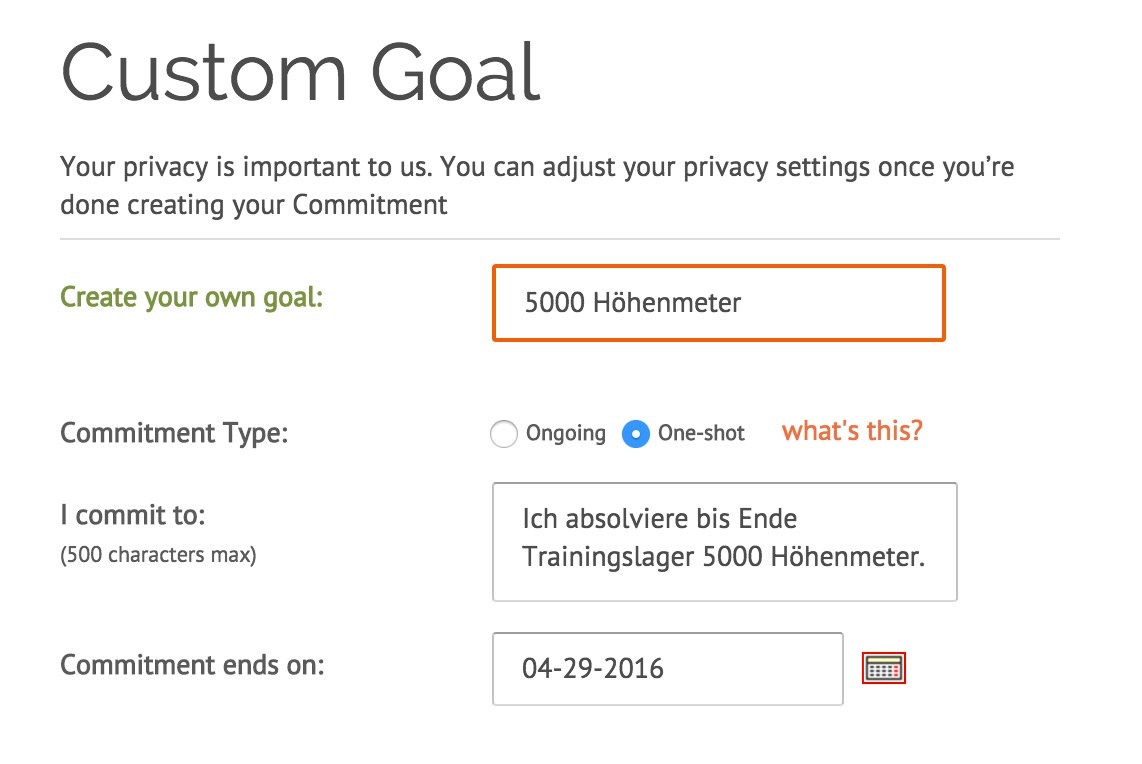
\includegraphics[width=0.7\textwidth]{figs/stickkcom.jpg}

  % ein url-Befehl in einer float"=Umgebung verlangt ein \protect
  \caption{Auf der Website \protect\url{http://www.stickk.com} lassen sich Ziele festlegen und darauf für sich selbst eine Wette abschliessen.
    Dass auch Geld gewettet werden kann, dass bei Nichterreichen futsch ist, soll das festhalten am Ziel erhöhen.}
  \label{fig:stickkcom}
\end{figure}




\subsection{Regenration vernachlässigen}

\subsection{Ernährung vernachlässigen}

Auch zur Regeneration gehört die richtige Ernährung.
Vielleicht im Rahmen eines TL ein Punkt, den man gerne etwas schleifen lässt.
Schliesslich hat man Ferien und treibt viel Sport -- entsprechend der Hunger.
Eine Woche reicht sicher nicht, um die Ernährung \emph{umzustellen}.
Aber vielleicht ist gerade diese Woche ideal, um die Sporternährung zu optimieren.

\subsection{Den Trainingsreiz nicht optimal in die Form retten}


\bibliographystyle{apacite}
% \bibliography{trainingslager.bib}
\bibliography{roadbikebib/roadbike.bib}

\end{document}
